\chapter{Pengantar Kecerdasan Buatan}
\label{chap:intro}

Selamat datang di dunia Kecerdasan Buatan (Artificial Intelligence/AI). Bab ini akan membawa Anda memahami apa sebenarnya AI itu, mengapa ia menjadi sangat populer belakangan ini, dan bagaimana ia berbeda dari teknologi komputer yang sudah kita kenal sebelumnya.

\section{Apa Itu Kecerdasan Buatan?}

Secara sederhana, **Kecerdasan Buatan (AI)** adalah kemampuan mesin atau komputer untuk meniru fungsi kognitif manusia, seperti belajar, memecahkan masalah, dan mengambil keputusan. Jika kalkulator adalah alat hitung yang pasif, AI adalah alat hitung yang bisa "belajar" dari pola angka yang Anda masukkan.

\begin{tipbox}
\textbf{Analogi Sederhana:}
Bayangkan Anda mengajari seorang anak kecil membedakan gambar kucing dan anjing.
\begin{itemize}
    \item \textbf{Pemrograman Tradisional:} Anda memberi tahu anak itu aturan kaku: "Jika punya kumis dan telinga lancip, itu kucing." (Masalah: Anjing juga bisa punya ciri ini).
    \item \textbf{AI (Machine Learning):} Anda menunjukkan 1.000 foto kucing dan 1.000 foto anjing, lalu membiarkan anak itu menemukan polanya sendiri.
\end{itemize}
\end{tipbox}

\section{Sejarah Singkat AI}

AI bukanlah konsep baru. Ia telah mengalami pasang surut yang panjang.

\begin{itemize}
    \item \textbf{1950 - Alan Turing:} Mengusulkan "Turing Test" untuk mengukur kecerdasan mesin.
    \item \textbf{1956 - Dartmouth Workshop:} Istilah "Artificial Intelligence" pertama kali dicetuskan.
    \item \textbf{1997 - Deep Blue:} Komputer IBM mengalahkan juara dunia catur Garry Kasparov.
    \item \textbf{2012 - AlexNet:} Terobosan dalam pengenalan gambar menggunakan Deep Learning.
    \item \textbf{2017 - Transformer Paper:} Google merilis paper "Attention is All You Need", fondasi dari ChatGPT.
    \item \textbf{2022 - ChatGPT:} AI Generatif meledak ke publik.
\end{itemize}

\section{Tiga Tipe AI}

Saat ini, kita sering mendengar istilah-istilah yang membingungkan. Mari kita luruskan.

\subsection{1. Artificial Narrow Intelligence (ANI)}
Ini adalah AI yang kita miliki sekarang. Ia sangat jago dalam satu tugas spesifik, tapi bodoh dalam hal lain.
\begin{itemize}
    \item \textbf{Contoh:} Google Maps, Face ID, Rekomendasi Netflix, AlphaGo.
    \item AlphaGo bisa mengalahkan juara dunia Go, tapi ia tidak tahu cara mengikat tali sepatu atau cara memesan pizza.
\end{itemize}

\subsection{2. Artificial General Intelligence (AGI)}
Ini adalah "Cawan Suci" riset AI. AGI adalah mesin yang memiliki kecerdasan setara manusia dalam segala bidang. Ia bisa belajar fisika, menulis puisi, dan memperbaiki kode programnya sendiri tanpa instruksi spesifik. Saat ini, AGI masih berupa teori dan fiksi ilmiah, meskipun model seperti GPT-4 mulai menunjukkan percikan kemampuan umum.

\subsection{3. Artificial Super Intelligence (ASI)}
Kecerdasan yang melampaui manusia tercerdas sekalipun dalam segala bidang. Ini adalah konsep futuristik yang sering dibahas dalam konteks etika dan keamanan jangka panjang.

\section{Machine Learning vs. Deep Learning vs. Generative AI}

Diagram berikut menjelaskan hubungan antara istilah-istilah ini:

\begin{center}
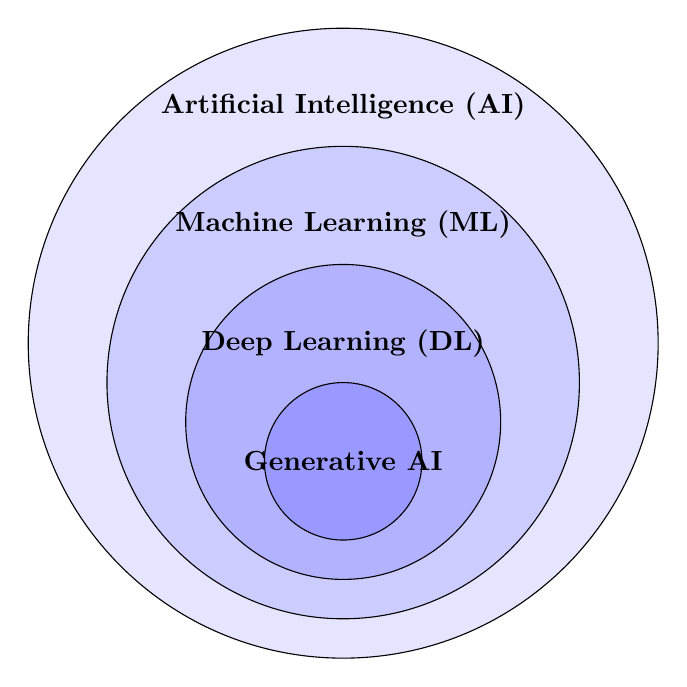
\begin{tikzpicture}
    \draw[fill=blue!10] (0,0) circle (4cm) node[yshift=3cm] {\textbf{Artificial Intelligence (AI)}};
    \draw[fill=blue!20] (0,-0.5) circle (3cm) node[yshift=2cm] {\textbf{Machine Learning (ML)}};
    \draw[fill=blue!30] (0,-1) circle (2cm) node[yshift=1cm] {\textbf{Deep Learning (DL)}};
    \draw[fill=blue!40] (0,-1.5) circle (1cm) node {\textbf{Generative AI}};
\end{tikzpicture}
\end{center}

\begin{itemize}
    \item \textbf{AI:} Konsep payung besar.
    \item \textbf{Machine Learning:} Bagian dari AI yang belajar dari data tanpa diprogram secara eksplisit.
    \item \textbf{Deep Learning:} Teknik ML yang menggunakan "Jaringan Saraf Tiruan" (Neural Networks) berlapis-lapis, terinspirasi dari otak manusia.
    \item \textbf{Generative AI:} Bagian dari Deep Learning yang bisa \textit{menciptakan} konten baru (teks, gambar, audio), bukan sekadar menganalisis data lama.
\end{itemize}

\section{Latihan Praktis 1: Audit AI Harian Anda}

\begin{exercisebox}
Ambil kertas atau buka aplikasi catatan di ponsel Anda. Selama 10 menit ke depan, catat semua interaksi Anda dengan teknologi hari ini dan coba identifikasi mana yang menggunakan AI.

\textbf{Contoh:}
\begin{itemize}
    \item Membuka kunci HP dengan wajah $\rightarrow$ AI (Computer Vision).
    \item Mencari resep di Google $\rightarrow$ AI (Search Ranking Algorithm).
    \item Menonton TikTok $\rightarrow$ AI (Recommendation Engine).
    \item Mengetik pesan dan muncul saran kata berikutnya $\rightarrow$ AI (Predictive Text).
\end{itemize}

\vspace{0.5cm}
\textbf{Tujuan:} Menyadari bahwa AI sudah menjadi bagian tak terpisahkan dari hidup kita, jauh sebelum ChatGPT muncul.
\end{exercisebox}
